% ICCIDS 2027 submission -- IEEE two-column conference format, 6 pages maximum.
% Build: pdflatex iccids2027 (twice), or tectonic iccids2027.tex
\documentclass[conference]{IEEEtran}
\IEEEoverridecommandlockouts

\usepackage{cite}
\usepackage{amsmath}
\usepackage{newtxtext,newtxmath}
\usepackage{graphicx}
\usepackage{booktabs}
\usepackage{tikz}
\usetikzlibrary{positioning,arrows.meta}
\usepackage{url}
\def\BibTeX{{\rm B\kern-.05em{\sc i\kern-.025em b}\kern-.08em
    T\kern-.1667em\lower.7ex\hbox{\sc e}\kern-.125em\hbox{X}}}

\begin{document}

\title{Blind-Gated Agentic Annotation for Evidence-Grounded Causal Knowledge Graphs of Protest Events}

% TODO before submission: confirm the author list, affiliations and e-mail addresses.
\author{\IEEEauthorblockN{Aditya Mohan Shenoy}
\IEEEauthorblockA{\textit{Department / Institution (to be completed)} \\
City, India \\
e-mail (to be completed)}
}

\maketitle

\begin{abstract}
Machine-coded event databases such as GDELT record \emph{what} happened, but not \emph{why}.
We show that inferring causes from their metadata fails: on 2024 Indian protest events, a
co-occurrence scorer kept shuffled event pairs as often as real ones (4.0\% versus 3.8\% at its
``pattern'' grade), and none of the 322 candidates it retrieved was a cause supported by the source
text. We therefore build causal links from the article text itself. A pipeline of large language
model (LLM) agents extracts events and grievances as verbatim text spans, merges duplicates,
proposes candidate causes, and judges each one under a written rubric that demands an exact quote.
Because no person can review thousands of links, every AI-accepted link must also pass a
\emph{blind} re-check by a fresh judge, calibrated with decoys; cycles are adjudicated by an agent,
and node merges respect cannot-link constraints from human verdicts. On a 300-article pilot, a
complete human review found that the blind re-check never accepted a link the person later rejected
(0 of 148). Scaled to 2{,}000 articles with no human in the loop, the system produced a graph of
1{,}416 sourced links explaining 358 protests. A random human spot check of 100 AI-only links found
89 of 99 correct (95\% CI 82--94\%): every link with explicit causal wording (69/69), but only two
thirds of links resting on implied evidence (20/30). A stricter AI pass could not separate the
wrong implied links, so the system exposes evidence type and hides unchecked implied links by
default.
\end{abstract}

\begin{IEEEkeywords}
causal knowledge graphs, large language models, agentic annotation, LLM-as-a-judge, event data,
GDELT, protest events, human-in-the-loop evaluation
\end{IEEEkeywords}

\section{Introduction}
Event databases such as GDELT~\cite{gdelt} and ACLED~\cite{acled} turn news into structured
records, and analysts routinely ask them causal questions: why did farmers march on Delhi in
February 2024, and what did the killing of a trainee doctor in Kolkata lead to? The records cannot
answer. They carry actors, CAMEO event codes~\cite{cameo}, places and dates, so any causal claim
built on them rests on co-occurrence, which machine-coded data already make noisy~\cite{hammond}.
News articles, in contrast, often \emph{state} causes (``protesting against'', ``in response to'',
``after'').

This paper describes a system that builds a causal knowledge graph~\cite{hogan} from those
statements and only from them. Every link carries the exact sentence that supports it, its source
URL, dates, and the full history of who judged it. The labelling is done by LLM agents, which makes
scale affordable but raises the question every LLM-as-a-judge study faces~\cite{zheng,wangfair}:
how far can the judgements be trusted when no person checks them?

Our contributions are:
\begin{itemize}
\item \textbf{A negative result} that motivates the design: a fused metadata scorer over GDELT
cannot tell real cause--effect pairs from shuffled ones, and retrieves no text-supported cause.
\item \textbf{An agentic, evidence-grounded pipeline} in which every extracted field is a verbatim
span and every causal link needs a mechanically verified quote, with rejected candidates kept as
hard negatives.
\item \textbf{Blind gating} as a substitute for human review: a second, blind judge with decoys,
calibrated against a complete human review, together with agent-adjudicated cycles and merges
constrained by human verdicts.
\item \textbf{Two recovery steps} for causes that retrieval misses, including turning causes that
an article states but extraction missed into new graph nodes.
\item \textbf{A human-measured precision} for the AI-only links, broken down by evidence type,
and a pre-registered test showing that a stricter AI judge does not fix the residual errors.
\end{itemize}

\section{Related Work}
\textbf{Event data.} GDELT~\cite{gdelt} codes events from global news with the CAMEO
ontology~\cite{cameo}; ACLED~\cite{acled} codes political violence and protest by hand. Studies of
machine-coded data report duplicate and mis-located events that limit micro-level
analysis~\cite{hammond}. Event knowledge graphs such as EventKG~\cite{eventkg} link events across
sources but do not encode why they happened.

\textbf{Causal relation extraction.} Corpora such as BECauSE~\cite{because} and Causal-TimeBank
\cite{mirza} annotate causal language within sentences; surveys cover pattern-based, statistical
and neural extractors~\cite{yangsurvey}. Mining news for causal event pairs has been used for
prediction~\cite{radinsky}. These works link mentions within a document; we link canonical,
cross-article events and conditions into multi-level chains, with each link traceable to a quote.

\textbf{LLMs as annotators and judges.} LLMs can match or exceed crowd workers on text
annotation~\cite{gilardi} and can stand in for human evaluation~\cite{chiang}, but LLM judges show
position and self-preference biases~\cite{zheng,wangfair}. We treat the LLM judge as a component
whose precision must be measured against people, and we report where it fails.

\section{Pipeline}
Fig.~\ref{fig:pipeline} summarises the stages. All model calls were made by LLM agents running
under written briefs; embeddings came from a locally run \texttt{all-mpnet-base-v2} sentence
encoder~\cite{sbert}. Each stage writes versioned, hashed artefacts and never overwrites them.

\begin{figure}[t]
\centering
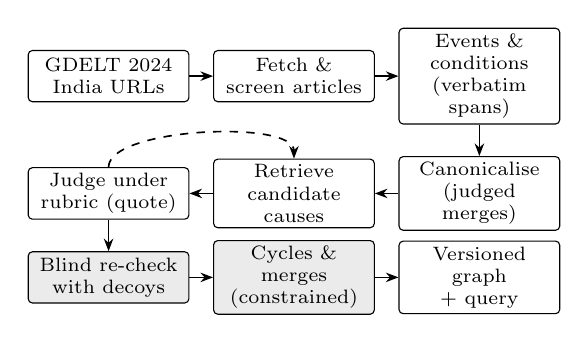
\begin{tikzpicture}[
  box/.style={draw, rounded corners=1.5pt, align=center, font=\scriptsize,
              minimum height=6.5mm, text width=19mm, inner sep=2pt},
  gate/.style={box, fill=black!8},
  arr/.style={-{Stealth[length=1.6mm]}, semithick}]
\node[box] (a) {GDELT 2024\\India URLs};
\node[box, right=3mm of a] (b) {Fetch \&\\screen articles};
\node[box, right=3mm of b] (c) {Events \& conditions\\(verbatim spans)};
\node[box, below=4mm of c] (d) {Canonicalise\\(judged merges)};
\node[box, left=3mm of d] (e) {Retrieve\\candidate causes};
\node[box, left=3mm of e] (f) {Judge under\\rubric (quote)};
\node[gate, below=4mm of f] (g) {Blind re-check\\with decoys};
\node[gate, right=3mm of g] (h) {Cycles \& merges\\(constrained)};
\node[box, right=3mm of h] (i) {Versioned graph\\+ query};
\draw[arr] (a) -- (b); \draw[arr] (b) -- (c); \draw[arr] (c) -- (d);
\draw[arr] (d) -- (e); \draw[arr] (e) -- (f); \draw[arr] (f) -- (g);
\draw[arr] (g) -- (h); \draw[arr] (h) -- (i);
\draw[arr, dashed] (f.north) .. controls +(0,0.5) and +(0,0.5) .. (e.north);
\end{tikzpicture}
\caption{Pipeline. Dashed: accepted causes become new targets, to a depth of three. Shaded
stages replace the human review of the pilot when the system runs without a person.}
\label{fig:pipeline}
\end{figure}

\subsection{Corpus and Screening}
We start from GDELT event records for India in 2024 and fetch the source articles, extracting text
with a production fetcher. Articles are drawn in a fixed, seeded hash order: a 300-article pilot,
then the next 1{,}700 for the scale-up. An LLM agent screens each article for protest relevance and
marks its focal event with supporting sentences. Of 2{,}000 articles, 915 were kept as protest
stories.

\subsection{Event and Condition Extraction}
A rule-based extractor over a spaCy~\cite{spacy} parse proposes event mentions in which every field
(action, actors, targets, place, time) is a character span of the article. An LLM reviewer accepts,
corrects or rejects each proposal and adds missed events; values that are not verbatim in their
sentence are dropped automatically, and spans are validated against a hash of the article text.
Grievances and standing states (a policy in force, unpaid dues, a water crisis) are extracted as
\emph{conditions} with a validity window, because the pilot showed that most missed causes are
conditions rather than events. The scale-up produced 7{,}083 event mentions and 1{,}146 condition
mentions.

\subsection{Canonicalisation}
Mentions of the same real-world event in different articles must become one node. Candidate pairs
are scored by embedding similarity, time overlap and word overlap; the score only orders review.
An agent judges every pair above a high band and a seeded sample below it, under a rubric that keeps
reports of an ongoing campaign on different dates apart. Judged-same pairs are joined by union-find,
and a grown cluster keeps the smallest earlier identifier so that prior verdicts stay attached. The
scale-up judged 8{,}913 event pairs and 2{,}661 condition pairs, giving 6{,}152 events and 810
conditions.

\subsection{Candidate Retrieval}
For each protest seed, any event dated up to seven days before it (or still under way) is proposed
if it shares the article, actor or place words, or has sentence similarity $\ge 0.45$; older events
need stronger signals (180-day window), and conditions qualify while in force. These signals only
propose candidates; none counts as evidence. To bound cost, all same-article candidates are kept and
the top eight from other articles per target.

\subsection{Causal Judging}
Each packet shows one effect, the full articles that report it, and its candidates, without
retrieval scores. The judge accepts a candidate only when the text states or plainly shows the link
(``over'', ``in response to'', ``protesting against'', an earlier stage of the same dispute, the call
that organised it), never on timing or shared topic. An accept carries one of five relations
(\textsc{triggers}, \textsc{motivates}, \textsc{mobilizes}, \textsc{escalates},
\textsc{prompts\_response}), a strength from 1 to 3, an evidence type (explicit wording or implied),
and an exact quote that is checked character for character against the shown text. A reject
carries one of eight reasons, for example \textsc{correlated\_only}, \textsc{wrong\_direction},
\textsc{temporally\_invalid} or \textsc{duplicate\_event}. Judges also list causes the article states
that no candidate represents. A quarter of the seeds are judged twice, independently, and agreement
is reported as Cohen's $\kappa$~\cite{cohen}. Accepted causes become the next targets, to a depth of
three.

\subsection{Graph Compilation}
The store is append-only and the compiler is deterministic: the same inputs give a byte-identical
graph whose SHA-256 is its version. Three rules matter.

\textbf{Precedence and the blind gate.} A person's verdict outranks every AI judgement. Without
one, an AI-accepted claim stays only if a \emph{blind} judge, who sees neither earlier votes nor the
chosen quote, accepts it again. Blind packets mix the accepted claims 1:1 with earlier rejects for
the same effects, as decoys, so that a judge who accepts everything is visible.

\textbf{Constrained merges.} Duplicate graph nodes are judged pairwise, and the latest decision per
pair wins. A merge is skipped if it would put both ends of a person-accepted link into one node, a
cannot-link constraint in the sense of constrained clustering~\cite{wagstaff}.

\textbf{Cycles.} A cause cannot be its own effect, so every cycle, found with Tarjan's
algorithm~\cite{tarjan} on the merged graph, holds a wrong link. A fixed rule (cut the weakest
link) cut correct links in our tests, so a fresh agent reads each cycle's evidence and names the
link whose quote does not support it.

\section{Evaluation Protocol}
We evaluate in two phases. In the \textbf{pilot} (300 articles), a person reviewed every link of the
AI-built graph, which calibrates the blind gate. In the \textbf{scale-up} (2{,}000 articles), no person
reviewed links during construction; afterwards the owner reviewed a seeded random sample of 100
AI-only links on a web form that showed each link's nodes, quoted evidence and AI verdicts. Confidence intervals are
Wilson score intervals~\cite{wilson}. Before the pilot, we also measured a GDELT metadata scorer
with negative controls: real pairs against shuffled pairs from unrelated stories and
future-dated pairs.

\section{Results}

\subsection{Metadata Alone Cannot Find Causes}
A scorer fusing six channels over GDELT records, including actor overlap, CAMEO-code
co-occurrence and lag, kept 5.4\% of
1{,}147 real pairs, 4.0\% of 557 shuffled pairs and 3.1\% of 1{,}058 future pairs. Its ``pattern''
grade fired on 3.8\% of real and 4.0\% of shuffled pairs, so it carries no signal. When AI judges
read the articles behind 322 candidates it retrieved for 23 targets, none was a cause the text
supports. The text pipeline, by contrast, accepted 0 of 60 shuffled and 0 of 35 valid future
controls in a blind test, while re-accepting 27 of 32 known positives.

\subsection{Pilot: A Complete Human Review}
The pilot graph had 207 links from 2{,}748 judged candidates (double-annotation $\kappa$ 0.78--0.93).
A blind re-check accepted 148 and rejected 59. The owner then reviewed all 207 and rejected 31,
so 15\% of the AI's accepted links were wrong. \textbf{All 31 rejected links were among the 59 the
blind judge had rejected}; the person rejected none of the 148 blind-accepted links, while
overturning 28 blind rejections (Table~\ref{tab:calib}). A blind accept is therefore strong evidence;
a blind reject is close to a coin flip. Against 103 causes documented by 67 independent sources, the
pilot recovered 25\% strictly and 43\% including partial matches; for half of the documented
causes the graph had no node at all, mostly because the 139-article corpus never reports them.

\begin{table}[t]
\caption{Calibrating the Blind Gate}
\label{tab:calib}
\centering
\footnotesize
\begin{tabular}{@{}lrr@{}}
\toprule
& Blind accept & Blind reject \\
\midrule
\multicolumn{3}{@{}l}{\emph{Pilot: person's verdict on 207 AI-accepted links}} \\
Person accepted & 148 & 28 \\
Person rejected & 0 & 31 \\
\midrule
\multicolumn{3}{@{}l}{\emph{Scale-up: no person, decoys mixed 1:1}} \\
AI-accepted links (1{,}352) & 1{,}209 (89\%) & 143 \\
Earlier rejects as decoys (1{,}352) & 44 (3\%) & 1{,}308 \\
\bottomrule
\end{tabular}
\end{table}

\subsection{Scale-up Without a Person}
Table~\ref{tab:funnel} gives the scale-up funnel and Table~\ref{tab:levels} shows the judging at each depth. Agreement stayed high
($\kappa$ 0.82--0.89). The blind gate removed 143 of 1{,}352 AI accepts, and accepted only 3\% of
decoys, against 9\% in the pilot, so the blind judges were not accepting what they were shown.
Across all rounds, 20{,}129 candidate claims were judged.

Recall here is the share of causes an article states that some candidate represented. Judges see
only candidates not yet judged, so a cause already linked looked ``missed''; correcting for links
already in the graph (embedding match $\ge 0.5$) raises the estimate, as shown.

\begin{table}[t]
\caption{Scale-up Funnel}
\label{tab:funnel}
\centering
\footnotesize
\begin{tabular}{@{}lr@{}}
\toprule
Stage & Count \\
\midrule
Articles screened / kept as protest stories & 2{,}000 / 915 \\
Event mentions / distinct events & 7{,}083 / 6{,}152 \\
Condition mentions / distinct conditions & 1{,}146 / 810 \\
Same-event pairs judged / judged same & 8{,}913 / 1{,}970 \\
Candidate cause claims judged (all rounds) & 20{,}129 \\
Protest seeds / with at least one cause & 373 / 358 \\
Links / nodes in the final graph & 1{,}416 / 1{,}188 \\
\bottomrule
\end{tabular}
\end{table}

\begin{table}[t]
\caption{Causal Judging in the 2{,}000-Article Scale-up}
\label{tab:levels}
\centering
\footnotesize
\begin{tabular}{@{}lrrrc@{}}
\toprule
Depth & Judged & Accepted & $\kappa$ & Stated-cause recall \\
\midrule
1 & 5{,}002 & 639 & 0.89 & 0.82 $\rightarrow$ $\sim$0.93 \\
2 & 5{,}822 & 464 & 0.82 & 0.74 $\rightarrow$ $\sim$0.82 \\
3 & 1{,}726 & 127 & 0.88 & 0.78 $\rightarrow$ $\sim$0.82 \\
\bottomrule
\end{tabular}
\end{table}

\textbf{Cycles and merges.} The blind gate alone removed three of the first four cycles. In total
the cycle adjudicator cut eleven links; most quoted a different event than the one they pointed to,
or had been judged against a node that a later merge changed. Pairwise node judging covered
16{,}604 pairs, every pair with similarity $\ge 0.6$, and merged 151 duplicates; a re-read of the
largest pass reversed 4 of its 77 ``same'' calls. The cannot-link rule blocked 5 merges, all of which would have
joined the unions' announcement of a march with the march itself, which a person had kept apart.

\subsection{Recovering Causes That Retrieval Missed}
The judges' lists of missed causes became a work queue (Table~\ref{tab:rescue}). Matching a missed
cause against the target's unjudged candidates, then against every event in the corpus, recovered
few links: the closest candidates were usually protests \emph{about} the cause, not the cause. The
real gap was extraction. Agents therefore turned each still-missing cause into a new event or
condition, every field a verbatim span of the sentence that states it; an undated new cause takes
no date later than the effect the article says it caused. These links were judged and blind-gated
like any other, and blind judges were told that an effect is the event its own fields name, since a
new node shares its sentence with the protest it caused. Searching the new nodes' own causes then
converged: the last round judged 113 candidates and accepted 3.

\begin{table}[t]
\caption{Recovery Rounds (claims judged / accepted / kept by blind gate)}
\label{tab:rescue}
\centering
\footnotesize
\begin{tabular}{@{}lrrr@{}}
\toprule
Round & Judged & Accepted & Kept \\
\midrule
Missed causes, target's pool & 334 & 63 & 54$^{\ast}$ \\
Missed causes, whole corpus & 691 & 39 & 36 \\
Stated causes as new nodes & 177 & 145 & 138 \\
Causes of the new nodes & 1{,}369 & 54 & 41 \\
Stated causes, second pass & 24 & 19 & 19 \\
\bottomrule
\multicolumn{4}{@{}p{0.92\columnwidth}@{}}{\scriptsize $^{\ast}$Depth 1: 220 judged, 36 accepted, 29
kept; depths 2--3: 114, 27, 25. Decoy acceptance in these blind passes ranged from 0\% to 11\%.}
\end{tabular}
\end{table}

The final graph has 1{,}416 links over 1{,}188 nodes, explains 358 of 373 protest seeds (57 in the
pilot), has no cycles, and rebuilds byte for byte. A typical chain, both links verified by a person,
runs from the farmers' \emph{Delhi Chalo} march (13 February 2024) through the leaders' 3 March call
to the 10 March \emph{rail roko}. The first link (\textsc{escalates}) rests on ``the two forums to
spread this agitation countrywide call upon the farmers and labourers across the country'', the
second (\textsc{mobilizes}) on ``a `rail roko' protest called by the Samyukta Kisan Morcha
(Non-Political) and the Kisan Mazdoor Morcha''; each quote links to its source article. Of 1{,}020 distinct causes reported missing by
the main judging rounds, 92 remained uncovered after recovery.

\subsection{How Accurate Are the AI-Only Links?}
Table~\ref{tab:spot} gives the person's verdicts on 100 random AI-only links. Overall precision is
89/99 (90\%; 95\% CI 82--94\%; one unsure). The errors are concentrated: \textbf{every link backed by
explicit causal wording was right} (69/69, an error rate below about 4\% at 95\% confidence), while a
third of links resting on implied evidence were wrong. Six of the ten errors were
\textsc{escalates} links, mostly joining two reports of the same ongoing protest or event; the
others quoted only one side of the link, or a different event than the node.

\begin{table}[t]
\caption{Human Spot Check of 100 Random AI-Only Links}
\label{tab:spot}
\centering
\footnotesize
\begin{tabular}{@{}lr@{}}
\toprule
Subset & Correct / decided \\
\midrule
All links & 89 / 99 (90\%) \\
Explicit causal wording & 69 / 69 \\
Implied evidence only & 20 / 30 \\
Depth 1 / 2 / 3 & 48/49, 33/42, 8/8 \\
From retrieval / rescue / stated-cause nodes & 79/89, 4/4, 6/6 \\
\bottomrule
\end{tabular}
\end{table}

\textbf{Can a stricter AI judge find the wrong implied links?} We re-judged all 285 unchecked
implied links under a stricter brief (both sides must appear in a quote; two reports of one
campaign are duplicates), with the 31 spot-checked implied links mixed in unmarked. We fixed the bar
in advance: reject at least 6 of the person's 10 rejects and keep at least 16 of the 20 accepts. The
strict judge rejected 8 of 10 but kept only 6 of 20; it keeps 30\% of good links and 20\% of bad
ones, so it was not applied. No simple rule helps either: implied \textsc{escalates} links split 5
correct, 5 wrong. The deployed query service therefore hides unchecked implied links by default and
shows each link's evidence type and whether a person checked it.

\section{Discussion and Limitations}
\textbf{What the gate buys.} The blind re-check is cheap and its accepts are trustworthy in both
phases, but it shares the first judge's blind spot: both read implied links as present. A third
judge with the same training does not fix this, which is consistent with known self-preference in
LLM judges~\cite{wangfair}. Evidence type, which the judge reports itself, is the best predictor of
error we found, and it is cheap to expose to users.

\textbf{Limitations.} (i) The scale-up's precision rests on a 100-link sample; about 900 explicit
AI-only links remain unchecked. (ii) A later pass in which the owner accepted all 285 implied links
in under three minutes is recorded as a fast pass, not a review, and is excluded from every number
above. (iii) Screening and extraction labels are AI-made and measured only against an independent
AI reading. (iv) Same-event pairs below the judged band were sampled, not judged, so some duplicate
events remain, and ongoing campaigns stay split by date. (v) Expansion stops at three levels, and
recall is bounded by what the corpus reports.

\section{Conclusion}
Causal questions over event data need text, not metadata. LLM agents can build a large,
evidence-grounded causal graph without a person in the loop, provided every link carries a verified
quote, accepts pass a blind, decoy-calibrated re-check, and structural repairs (cycles, merges)
defer to recorded human verdicts. On this corpus such links were 90\% correct, and every link with
explicit causal wording was correct. The remaining errors sit in implied links, where an AI judge
does not help and a person still does. The code, rubrics and graph are released at
\url{https://github.com/AdityaMohanShenoy/gdelt-knowledge-graph}.

\section*{Generative AI Disclosure}
LLM agents built on Anthropic Claude models, running in Claude Code, performed the data labelling
described in Sections~III--V: article screening, event and condition review, same-event judgements,
causal judging, blind re-checks, cycle adjudication and node-merge judgements. An OpenAI Codex agent
provided an independent second reading for pilot screening. The same Claude-based agent also wrote
the pipeline code with the author and drafted this manuscript's text, tables and figure from the
project's measurement reports. The author verified every number against those reports and is
responsible for the content. Human verdicts reported here were made by the author.

\begin{thebibliography}{00}
\bibitem{gdelt} K. Leetaru and P. A. Schrodt, ``GDELT: Global data on events, location, and tone,
1979--2012,'' in \textit{Proc. ISA Annu. Conv.}, 2013.
\bibitem{acled} C. Raleigh, A. Linke, H. Hegre, and J. Karlsen, ``Introducing ACLED: An armed
conflict location and event dataset,'' \textit{J. Peace Res.}, vol. 47, no. 5, pp. 651--660, 2010.
\bibitem{cameo} P. A. Schrodt, ``CAMEO: Conflict and mediation event observations event and actor
codebook,'' Pennsylvania State Univ., 2012.
\bibitem{hammond} J. Hammond and N. B. Weidmann, ``Using machine-coded event data for the
micro-level study of political violence,'' \textit{Res. \& Politics}, vol. 1, no. 2, 2014.
\bibitem{hogan} A. Hogan \textit{et al.}, ``Knowledge graphs,'' \textit{ACM Comput. Surv.}, vol. 54,
no. 4, pp. 71:1--71:37, 2021.
\bibitem{zheng} L. Zheng \textit{et al.}, ``Judging LLM-as-a-judge with MT-Bench and Chatbot Arena,''
in \textit{Proc. NeurIPS Datasets and Benchmarks Track}, 2023.
\bibitem{wangfair} P. Wang \textit{et al.}, ``Large language models are not fair evaluators,'' in
\textit{Proc. ACL}, 2024.
\bibitem{eventkg} S. Gottschalk and E. Demidova, ``EventKG: A multilingual event-centric temporal
knowledge graph,'' in \textit{Proc. ESWC}, 2018, pp. 272--287.
\bibitem{because} J. Dunietz, L. Levin, and J. Carbonell, ``The BECauSE corpus 2.0: Annotating
causality and overlapping relations,'' in \textit{Proc. Linguistic Annotation Workshop}, 2017,
pp. 95--104.
\bibitem{mirza} P. Mirza, R. Sprugnoli, S. Tonelli, and M. Speranza, ``Annotating causality in the
TempEval-3 corpus,'' in \textit{Proc. EACL Workshop Comput. Approaches to Causality in Language},
2014, pp. 10--19.
\bibitem{yangsurvey} J. Yang, S. C. Han, and J. Poon, ``A survey on extraction of causal relations
from natural language text,'' \textit{Knowl. Inf. Syst.}, vol. 64, pp. 1161--1186, 2022.
\bibitem{radinsky} K. Radinsky, S. Davidovich, and S. Markovitch, ``Learning causality for news
events prediction,'' in \textit{Proc. WWW}, 2012, pp. 909--918.
\bibitem{gilardi} F. Gilardi, M. Alizadeh, and M. Kubli, ``ChatGPT outperforms crowd workers for
text-annotation tasks,'' \textit{Proc. Natl. Acad. Sci.}, vol. 120, no. 30, e2305016120, 2023.
\bibitem{chiang} C.-H. Chiang and H.-y. Lee, ``Can large language models be an alternative to human
evaluations?'' in \textit{Proc. ACL}, 2023, pp. 15607--15631.
\bibitem{sbert} N. Reimers and I. Gurevych, ``Sentence-BERT: Sentence embeddings using Siamese
BERT-networks,'' in \textit{Proc. EMNLP-IJCNLP}, 2019, pp. 3982--3992.
\bibitem{spacy} M. Honnibal, I. Montani, S. Van Landeghem, and A. Boyd, ``spaCy: Industrial-strength
natural language processing in Python,'' Zenodo, 2020.
\bibitem{cohen} J. Cohen, ``A coefficient of agreement for nominal scales,'' \textit{Educ. Psychol.
Meas.}, vol. 20, no. 1, pp. 37--46, 1960.
\bibitem{wagstaff} K. Wagstaff, C. Cardie, S. Rogers, and S. Schr\"{o}dl, ``Constrained k-means
clustering with background knowledge,'' in \textit{Proc. ICML}, 2001, pp. 577--584.
\bibitem{tarjan} R. E. Tarjan, ``Depth-first search and linear graph algorithms,'' \textit{SIAM J.
Comput.}, vol. 1, no. 2, pp. 146--160, 1972.
\bibitem{wilson} E. B. Wilson, ``Probable inference, the law of succession, and statistical
inference,'' \textit{J. Amer. Statist. Assoc.}, vol. 22, no. 158, pp. 209--212, 1927.
\end{thebibliography}

\end{document}
